
\chapter{Case Study} \label{case_study}

The aim of this chapter is to present a case study using real data, providing a meaningful pipeline with the ability to demonstrate the application's features. This case study consists in the chemometric characterization of the carotenoid content in cassava roots tissue, using \gls{uv}, CIELAB data and a \acrlong{llf} of the two.


\section{Cassava}

\subsection{Introduction}

Cassava is the commonly used term to designate the \textit{Manihot esculenta} species. This tuberous-root plant species offers a wide variety of agronomic advantages, being resilient to droughts, inexpensive, resistant to major diseases and pests, easy to grow and having flexible harvest times, allowing farmers to harvest the roots as needed. It is, therefore, a valuable source of energy for people living in the poorest regions. However, cassava roots are a poor source of provitamin A carotenoids, whose deficiency is a major problem in such regions \citep{la2013biofortified, sanchez2014prediction}. 

Carotenoids are one of the most important natural pigments, having already been recognized benefits of carotenoid consumption such as the diminished risk of several degenerative disorders, including various types of cancer, cardiovascular or ophthalmological diseases, as well as their preventive effect associated with their antioxidant activity, protecting cells and tissues from oxidative damage \citep{stahl2003antioxidant}. However, only vitamin A precursors $\beta$-carotene, $\alpha$-carotene and $\beta$-cryptoxanthin represent the major sources of carotenoids in the human diet.

With a broad range of colors, varying from yellow to dark-red, carotenoids confer color to many plant leaves, fruits and flowers, as well as birds, insects, fish, and crustaceans. The color of cassava's starchy root, which can vary from white to red, is strongly correlated to the presence and contents of several carotenoid pigments and their associations \citep{sanchez2006reduction}. However, the possibility of adopting the color of roots as an indirect criterion for selection of higher carotene content is questionable, since color is a characteristic of difficult visual evaluation. Thus, the use of a standardized color measurement technique is of most importance.

The CIELAB color technique was adopted by the \gls{cie} and is based on the Lab color space, which describes mathematically all perceivable colors in three dimensions: L* for lightness and a* and b* for the color opponents green-red and blue-yellow. The values of these three variables are usually absolute, with the L* value representing the darkest black at L* = 0, and the brightest white at L* = 100. On the other hand, the a* value represents red and green opponents at positive and negative values, respectively, while the b* value represents yellow and blue opponents at positive and negative values, respectively \citep{brockes1982evaluation, schanda2007colorimetry}. A visual representation of the CIELAB color space is shown in \autoref{cielab}.

\begin{figure}[h]
	\centering
	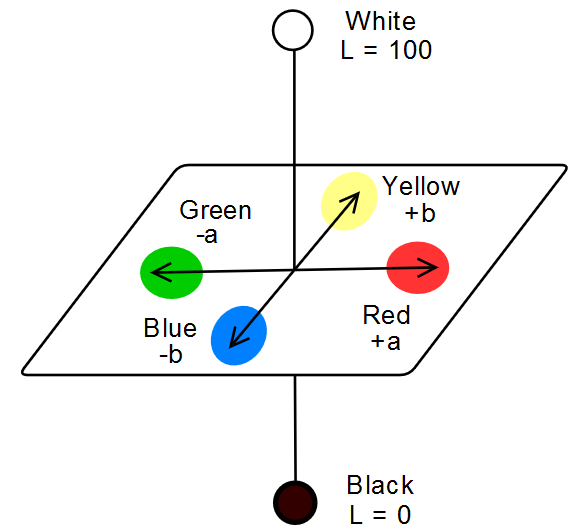
\includegraphics[width=0.4\linewidth]{Imagens/cielab}
	\caption{Representation of the CIE L* a* b* color space.}
	\label{cielab}
\end{figure}

Currently, CIELAB is the most used system for quantitative color description of an object, given its uniformity, ease of acquisition, very low cost and device independence. Considering that this technique facilitates the acquisition of measurements directly on the field, while also avoiding the degradation of the compounds, it becomes an appealing approach in comparison to traditionally used methods such as \gls{hplc} or \gls{uv}. The CIELAB color technique has been applied for instance in the unique identification of skin color for clinical and scientific purposes \citep{weatherall1992skin} and as an optimal color design approach for transforming patients' perception into color elements \citep{liu2014optimal}.

Combining \gls{uv} and CIELAB colorimetric data, the aim of the present case study is to validate a quantification method for carotenoid content estimation in roots of \textit{M. esculenta}, assuming that the statistical and machine learning techniques can correlate these data types, to ultimately detect genotypes of M. esculenta with high contents of carotenoids. Importantly, this study provides tools that can support the plant-breeding program at Epagri (Agricultural Research Company and Rural Extension of the State of Santa Catarina, \href{http://www.epagri.sc.gov.br/}{\nolinkurl{http://www.epagri.sc.gov.br/}}) that aims to obtain genotypes with high levels of pro-vitamin A carotenoids and superior nutritional traits.


\subsection{Ultraviolet-visible Data}

Fifty root samples of \textit{M. esculenta} genotypes harvested in 2015/2016 season from the Epagri's germplasm bank were used due to their economic and social importance. Samples were visually selected for high content in carotenoids with provitamin A activity and lycopene. 

After carotenoid extraction from the roots using organosolvents, extracts absorbances were then recorded using a spectral window from 200 to 700 $\eta m$. Aliquots of the extracts were also injected into a liquid chromatograph for carotenoid quantification purposes. 

Considering that most carotenoids exhibit absorption in the visible region of
the spectrum, between 400 to 500 $\eta m$, a subset of the original UV-visible
dataset with samples belonging to this wavelength interval was used. Missing values contained within this dataset were replaced with the mean of the variables' values.

In order to accurately predict the carotenoid contents in cassava roots regression-derived statistical and machine learning models were used, including \gls{pls}, decision trees, \gls{svm}s, random forests and neural networks. Three response variables were used in the machine learning approach: the \gls{tcc} determined by spectrophotometry (Lambert-Beer law), the \gls{tcc} and the content of trans-$\beta$-carotene, the most abundant carotene in cassava roots, both determined by HPLC.

Models that showed best performance were selected and the variable importance calculated. Various pre-processing methods were applied to the datasets to see whether model performance could be improved, using these models. The data was also subject to filter-based feature selection (40\%, 60\% and 80\% data filtering) to determine once again if it could improve model performance.


\subsection{CIELAB Data}

Immediately after harvest, color measurements of the root samples were made. For all fifty samples, three readings were performed at different sites.

The analysis pipeline was similar for the CIELAB dataset, however, models that included feature selection, the data pre-processing and filtering processes were excluded from the analysis pipeline, as it did not make sense to perform these, considering there are only 3 features in the dataset (L* a* and b* parameters), while pre-processing was meant for spectral data.

\subsection{Fusion Data}

For the fusion dataset, which contained 104 variables (absorbance values + L* a* b* parameters), the analysis pipeline was similar to that of the CIELAB dataset, while data filtering was also performed similarly to the \gls{uv} dataset.







